\section{Reuse and Warmstarting Optimizations}\label{sec-reuse-and-warmstarting}
With the experiment graph constructed and materialized, our collaborative optimizer looks for opportunities to reuse existing materialized artifacts in the experiment graph and warmstart model training operations.
Every artifact of the incoming workload DAG has one of the three following states: (1) the artifact does not exist in the Experiment Graph, (2) the artifact exist in the Experiment Graph but is not materialized, and (3) the artifact is materialized.
For the first two states, the client must execute the operations of the DAG to generate the artifact.
However, when the artifact is materialized, we can either load it from the Experiment Graph or let the client execute the operations.
Both loading the artifact and executing the operations incur costs.
In this section, we first describe our reuse algorithm that selects the a subset of the materialized artifacts which results in a DAG with lowest execution time, i.e., cost of loading and cost of computing all the artifacts of the workload DAG.
Reusing model artifacts 
Then, we discuss our warmstarting approach for model training operations.
Due to stochastic behavior of some model training operations, we can always directly reuse a materialized model.
Therefore, we opt to warmstart the training operation of the model artifact which leads to a decrease in training time.
%\begin{figure}
%\centering
%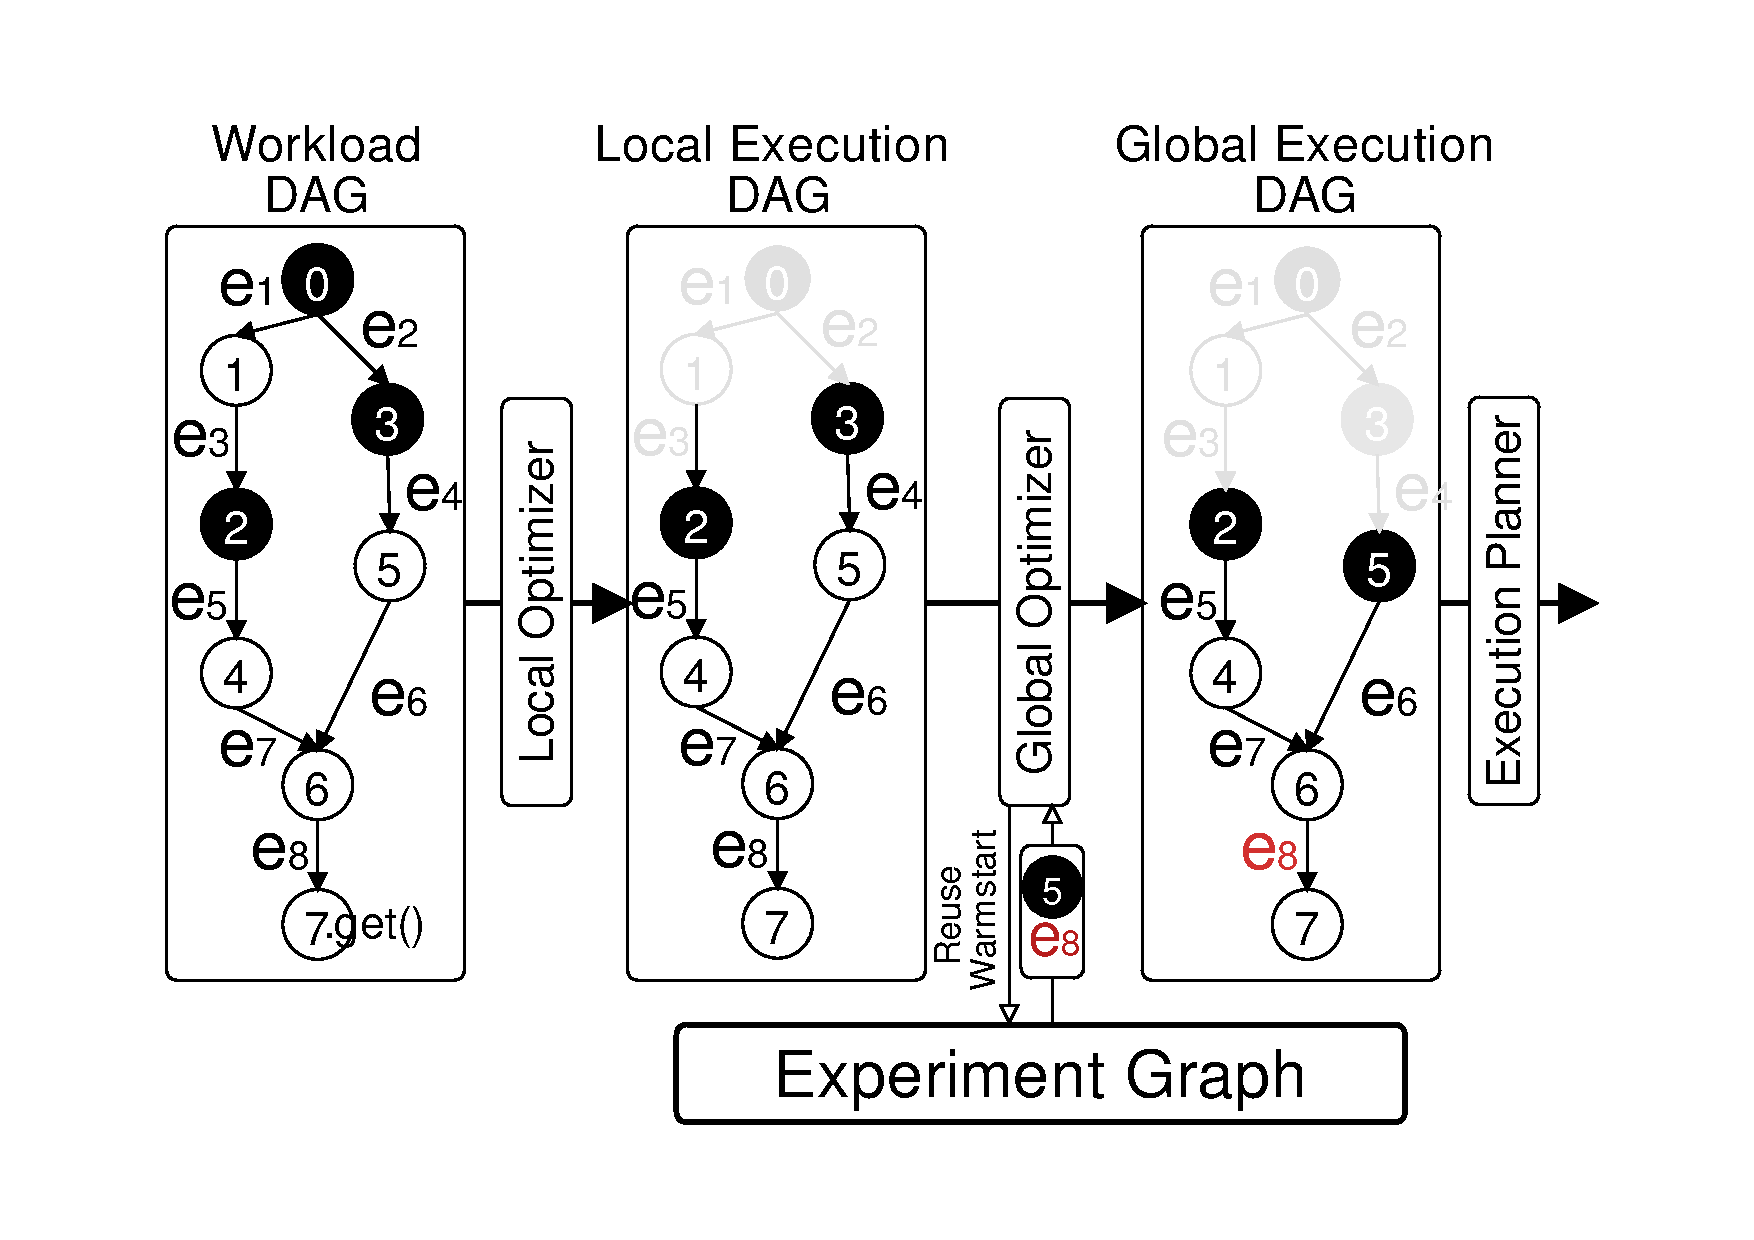
\includegraphics[width=\columnwidth]{../images/reuse-optimization}
%\caption{Reuse and Warmstarting Optimizations}
%\label{reuse-warmstart-figure}
%\end{figure}
%Figure \ref{reuse-warmstart-figure} shows an example of the optimization process for reuse and warmstarting.
%In the workload DAG, the user invokes the $.get()$ command on vertex 7, which represents a machine learning model.
%To compute the local execution DAG, the local optimizer scans the workload DAG to find previously computed vertices. 
%This is an important step for interactive workloads.
%In this example, besides from the root vertex (vertex 0), vertex 2 and 3 are already computed (represented by black color).
%Therefore, the local optimizer prunes vertex 0 and edges $e_1$ and $e_2$.
%Then, the global optimizer looks for reuse and warmstarting opportunities in the experiment graph.
%In this example, vertex 5 was computed in a previous workload and its result was materialized in the experiment graph.
%Similarly, the model training operation $e_8$ was already executed in an existing workload.
%The global optimizer transfers vertex 5 to the workload, which results in further pruning of vertex 3 and edge $e_4$.
%The global optimizer also warmstarts $e_8$ which increases the convergence rate of the training operation.
%Both Reuse and Warmstarting can reduce the total execution time of the workload.
%In the rest of this section, we present the details of both Reuse and Warmstarting methods.


\subsection{Reuse Algorithm} 
\textbf{Preliminaries.} 
We refer to the workload DAG as $WG$ and the Experiment Graph as $EG$.
For every vertex, $v \in WG$, we define $cost_l(v)$ as the cost (in seconds) of loading $v$ from $EG$  and $cost_c(v)$ as the computation of $v$ given its parent vertices in $WG$.
If an artifact exist in $EG$ but is not materialized, then we set $cost_l(v)=\inf$.
For artifacts that do not exist in $EG$, we set both $cost_l(v)$ and $cost_c(v)$ to unknown.
This is because these artifacts have never appeared in any workloads and we have no prior information about them.
Lastly, if an artifact is already computed in $WG$, such as the root artifacts or pre-computed artifacts in interactive workloads, we assign $cost_c(v)=0$, this is because the artifact is already available in the client's memory.

\textbf{Linear-time Algorithm.}
Our reuse algorithm comprised of two parts: forward-pass and backward-pass.
In forward-pass, the algorithm selects the set of materialized vertices to load from Experiment Graph into the workload DAG.
After the forward-pass, the inclusion of some vertices in the materialized set is not necessary since they will be pruned from the execution.
Therefore, the backward-pass removes all the unnecessary materialized vertices.
Algorithm \ref{algorithm-reuse} shows the details of our reuse algorithm.
For every vertex of $WG$, we store its total computation cost, i.e., computing the vertex from the sources, inside the $total\_cost$ dictionary.
In collaborative environments, the client always loads the source artifacts completely.
Therefore, we set their total cost to 0 (Lines 1 and 2).
Then, we visit every vertex in their topological order.
If the client program has already computed a vertex inside $WG$, then we set its total cost to 0 (Lines 5 and 6).
Otherwise, we compare load cost of the vertex with the cost of computing it from its parents and assign its total cost to the smaller of the two (Lines 8-14).
Note that vertices which are not materialized have a load cost of infinity, therefore, the algorithm will never load an unmaterialized vertex.

\begin{algorithm}[h]
\KwData {$WG$: workload DAG, $EG$: Experiment Graph}
\KwResult {$\mathcal{M}$: Set of materialized vertices}
\For {$s \in sources(WG)$}{
	$total\_cost[s] = 0$\;
}
$\mathcal{M} = \emptyset$\;
\For {$v \leftarrow topological\_order(WG)$}{
	\eIf{$v$ computed in $WG$}{
		$total\_cost[v]=0$\; 		
		}{
		$parents\_cost = \sum\limits_{p \in parents(v)} total\_cost[p]$\;
		$compute\_cost = cost_c(v) + parent\_cost$\;
		\eIf {$ cost_l(v) < compute\_cost$}{
			$total\_cost[v] = cost_l(v)$\;
			$\mathcal{M} = \mathcal{M} \cup v$\;
		}{
			$total\_cost[v] = compute\_cost$\;
		}
	}
}
\caption{Forward-pass Algorithm}\label{forward-pass}
\end{algorithm}
During the backward-pass, we visit every vertex of $WG$ in reverse of their topological order (from terminal to roots).
For every materialized vertex that we encounter, we add the vert
The algorithm visits each node only once, thus incurring a complexity of $\mathcal{O}(|V|)$ where $|V|$ is the number of vertices in $WG$.
Figure \ref{fig-reuse-algorithm} show an example of the reuse algorithm.


\begin{figure}
\centering
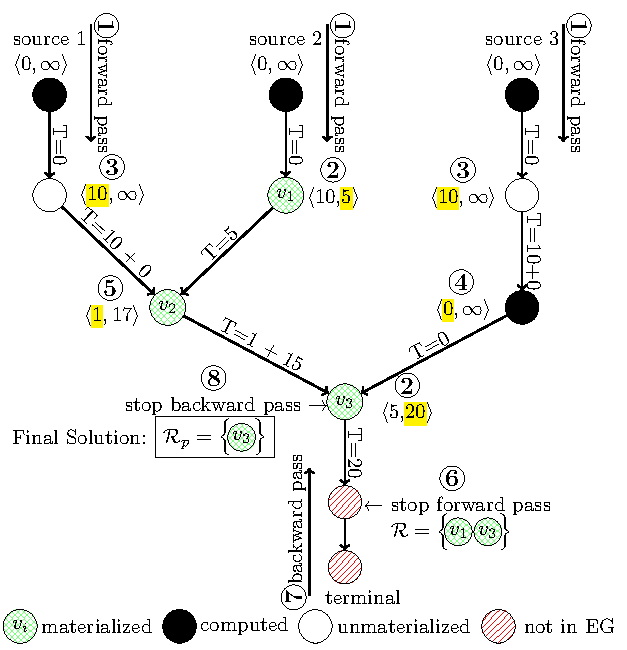
\includegraphics[width=\linewidth]{../images/tikz-standalone/reuse-algorithm}
\caption{Reuse Algorithm Example.}
\label{fig-reuse-algorithm}
\end{figure}


\textbf{Early-Stopping.} 
An artifact can exist in the Experiment Graph if and only if its parents also exist in the Experiment Graph.
Therefore, during the traversal of the workload DAG, if a vertex does not exist in the Experiment Graph, we can stop the traversal down that branch (Figre xxx). 
\subsection{Warmstarting}
Many model training operations include random processes.
For example, in random forests, to decide when to split a tree node, features are randomly permuted.
A random seed parameter controls the random behavior.
Two training operations on the same dataset with the same hyperparameters may result in completely different models if the random seeds are different.
Therefore, the Reuse algorithm is not able to find the previously trained model, if the random seeds are different.
Instead, we try to warmstart model training operations using the existing models in the experiment graph.
In warmstarting, instead of randomly initializing the parameters of a model before training, we initialize the model parameters to a previously trained model.
Warmstarting has shown to decrease the total training time \cite{baylor2017tfx}.

During the graph construction, for every model training operation, we compute an extra hash value, which does not consider the random seed parameter.
We refer to this hash value as the seedless hash.
The seedless hash allows us to find similar training operations that only differ in the random seed.
When the Reuse algorithm encounters a machine learning model vertex, two scenarios can occur.
In the first scenario, a similar model vertex with the same id also exists in the experiment graph. 
In this scenario, we can safely reuse the model vertex since the only way for both model vertices to have the same id is that both models are trained on the same data using the same training operations with the equal hyperparameters and random seeds.
In the second scenario, the machine learning model vertex does not exist in the experiment graph.
In this scenario, we utilize Algorithm \ref{algorithm-warmstarting} to detect whether warmstarting is possible.
The warmstarting algorithm receives the model vertex $v_m$, the local execution DAG, and the experiment graph as inputs and tries to warmstart the training operation for $v_m$ with a model from the experiment graph.
The algorithm first finds the parent of the model vertex, represented by $v_{dataset}$ on Line 1 and the training operation, represented by $e_{train}$ on Line 2.
$v_{dataset}$ is the dataset used in the operation $e_{train}$.
To warmstart $e_{train}$, the algorithm first ensures $v_{dataset}$ is in the experiment graph (Line 4).
Then, for every outgoing edge of the $v_{dataset}$, the algorithm compares the seedless hash of the edge with the seedless hash of $e_{train}$.
In the algorithm, the function $sl\_hash$ computes the seedless hash of an edge.
Equal seedless hashes indicate that the training operation from the experiment graph only differs in the random seed when compared to $e_{train}$.
Therefore, the result of the training operation in the experiment graph is a candidate for warmstarting $e_{train}$ (Lines 6-8).
In case there are more than one wamrstarting candidates, we select the candidate model with the maximum quality to warmstart the training operation (Lines 9-11).
\begin{algorithm}[h]
\KwData {$v_m$: model vertex, $G_L$: local execution DAG, $G_E$: experiment graph}
\KwResult {modified $G_L$ with warmstarted training} 
$v_{dataset} \coloneqq parent(G_L, v_m)$\;
$e_{train} \coloneqq edge(G_L, v_{dataset}, v_m)$\;
$\mathcal{C}\coloneqq \emptyset$\tcp*{set of candidate models}
\If{$v_{dataset} \in G_E$}{
	\For{$e \in out\_edges(G_E, v_{dataset})$}{
		\If {$sl\_hash(e) = sl\_hash(e_{train})$}{
			$m \coloneqq e.dest$\;
			$\mathcal{C}.add(m)$\;		
		}	
	}
}
\If{$\mathcal{C}.not\_empty()$}{
	$m \coloneqq \argmax\limits_{m \in \mathcal{C}} \text{ } quality(m)$\;
	$warmstart(e_{train}, m)$\;
}
\caption{Warmstarting}\label{algorithm-warmstarting}
\end{algorithm}